\chapter{The base model with environmental variability}\label{ch:2_base_model}

\begin{CJK}{UTF8}{min}
{\color{red}
本章は\cite{Inaba2025a}を博士論文用に編集して記載します。現時点 (プレ予備審査時点) では Model 以降をほぼそのまま貼り付けただけですが、予備審査までにできるだけ博論全体の中での流れを整えます。
}
\end{CJK}
\vspace*{1cm}

In this chapter, we develop a foundational model that serves as the basis for the analyses in Chapters 3 and 4, with the aim of examining how environmental variability (EV) influence the evolution of cooperation.

\section{Model}

We use an agent-based simulation model within the framework of evolutionary game theory to investigate how increasing EV influences the evolution of cooperation.
Given the limited availability of detailed data on EV and the spatial distribution of hominid groups during the MSA in Africa, our model adopts a highly abstracted approach, aiming to reveal the general effects of EV based on reasonable assumptions while excluding specific details.
The model operates as follows: several geographically separated regions, each with varying levels of resource accessibility, experience fluctuating resource availability over time (EV).
Each region hosts a single group (agent), and interactions between groups, such as resource exchanges (game) and behavioral pattern transmission (reformation), affect and adjust their relationships.

\subsection*{Agent and structure}

In this model, each agent represents a single group and has a strategy of either cooperation or defection (in this study, ``C" represents a cooperation strategy or a cooperator, while ``D" represents a defection strategy or a defector).
Initially, all agents are set to D, as intergroup cooperation is considered extremely unlikely \cite{DeDreu2022a, Rodrigues2023}.
This study focuses exclusively on intergroup interactions and does not consider intragroup interactions.
While a two-level model would be necessary to analyze the tension between intergroup and intragroup interactions, as seen in multilevel selection studies, a one-level model is suitable here given our focus on intergroup interactions.
All agents are suited within a geographic structure, forming an interaction structure.

The geographic structure is modeled as a line segment with periodic boundary conditions, represented visually as a circle (Fig \ref{fig:model}).
$N$ agents are evenly spaced along the circle.
Although a one-dimensional spatial structure is used for simplicity, more realistic structures can be explored as empirical studies progress.
Mobility is not considered in this study to keep the model simple as an initial approach.
We plan to incorporate mobility in future work, as it is reasonable to assume that a group might move to a resource-rich region when its resources become scarce.
However, the assumption of no mobility is not entirely unrealistic, as some studies have highlighted the tendency for settlement during the MSA \cite{Marean2010, Wadley2011, Kandel2012}.

The interaction structure defines the relationships between agents, which are not limited by the geographic arrangement.
These relationships affect the frequency of games (described later) and are subject to rewiring through reformations (also described later).
The network, where agents are represented as nodes and relationships as edges, is characterized as an undirected, unweighted, and dynamic graph.
The initial network is a regular network with a degree of $k = 4$.

\subsection*{EV}

The resource represents the amount of goods or wealth necessary for survival that a group (agent) can obtain from the natural environment (e.g., food, materials for stone tools required to gather food).
Resources are allocated to each agent at each time step, with the amount varying across different regions.
The node with the highest resource allocation is referred to as the source of resources (SoR).
The further an agent is located from the SoR geographically, the less resource it receives, as determined by the resource decrement factor, $f_{RD}$.
Specifically, the resource allocated to agent $i$ is calculated as $r_i = r_p - |i - p| f_{RD}$.
Here, $r_i$ represents the resource allocated to agent $i$, $p$ is the index of the SoR, and $|i - p|$ represents the distance between $i$ and $p$, accounting for the boundary conditions, rather than the usual absolute value.
Additionally, there is a universal resource threshold, $\theta$, for all agents; any agent falling below this threshold must reformulate its strategy and relationships.

In our study, EV to refers to resource variability, represented by stochastic models.
EV can be divided into variability in distribution of resources among regions and in total quantity of resources across all regions.
Although variations in resource types are also an important consideration, we simplify the model assuming a single resource type.
The two forms of variability are termed regional variability (RV) and universal variability (UV).
RV is a type of EV in which the distribution of resource-rich and resource-poor regions changes over time; specifically, the SoR moves randomly.
The SoR’s index $p_t$ at time $t$ fluctuates according to a stochastic process expressed as $p_{t+1} = ( p_t + \Delta_t ) \mod N$.
Here, $\Delta_t$ is a random integer step uniformly distributed within the range $[ -\sigma_R, \sigma_R ]$, where $0 \leq \sigma_R \leq N / 2$.
UV represents another form of EV in which the total resource quantity fluctuates randomly over time, while the resource distribution between regions remains fixed.
This variability reflects large-scale fluctuations in resource availability across a wide area encompassing all regions.
However, to simplify the implementation, we fix the resource values and instead model UV by varying the threshold value $\theta$, which determines when reformation occurs.
The fluctuation is modeled by an AR(1) process \cite{Hasselmann1976, Vyushin2012, Salcedo2022}, $\theta_{t+1} = \mu_\theta (1 - \beta) + \theta_t \beta + \epsilon$, where $\mu_\theta$ is the expected value of $\theta$, $\beta$ is the autoregressive coefficient ($0 \leq \beta \leq 1$), and $\epsilon$ is a normally distributed noise term with mean 0 and standard deviation (SD) $\sigma_\theta$.
The intensity of RV is determined by the shift range of the SoR ($\sigma_R$), while the intensity of UV is influenced by the autoregressive coefficient ($\beta$) and the SD of the noise term ($\sigma_\theta$).
We examine the impact of EV on the evolution of cooperation under three scenarios: RV, UV, and combined variability (CV), where both the SoR shifts and the threshold $\theta$ fluctuates.

\begin{figure}[ht]
    \centering
    \includegraphics[width=1.0\linewidth]{figures/2/Fig1}
    \caption[Relationships, geographical structure, and EV.]{
Relationships, geographical structure, and EV.
Each small circle within the gray circle represents a group (agent, node), with the number inside indicating the resource value.
The gray ring represents the geographical structure, and each line connecting agents denotes a relationship (edge).
(a) In the RV model, the SoR shifts randomly within the geographical structure, and resources are then allocated to other nodes.
Following this, the game and reformation processes occur.
The resource threshold for reformation is fixed at $\theta = 0.5$.
(b) In the UV model, the SoR remains fixed, but the threshold $\theta$ fluctuates randomly, following an AR(1) process.
    }
    \label{fig:model}
\end{figure}

\subsection*{Game}

Communication over resources (such as primitive bartering, giving, looting) between agents is represented by simple pairwise games.
These games can only be played with an opponent who is connected through a network edge.
The probability that agent $i$ selects agent $j$ as its game opponent from its neighbors is $p^G_{i,j} = \frac{1}{n}$;
$n$ is the number of neighbors of $i$, and neighbors refer to an agent directly connected to $i$ in the interaction structure network.
The game procedure follows a pairwise public goods game (PGG) \cite{Hardin1968, Binmore1994, Kollock1998, Santos2008} with resource threshold considerations.
First, assume that agent $i$ selects agent $j$.
If the agent is C, it contributes a surplus resource $M_i = \max(r_i - \theta, 0)$.
If the agent is D, it does not contribute any resource.
The contributed resources are multiplied by a factor $b$ ($1 \leq b \leq 2$) and then equally divided between $i$ and $j$.
The payoff table is as follows:
\begin{equation}
\begin{array}{|c|c|c|}
\hline
  & C & D \\
\hline
C & R_i, R_j & S_i, T_j \\
\hline
D & T_i, S_j & P_i, P_j \\
\hline
\end{array}
\end{equation}
\begin{align}
R_i &= \left(\frac{b}{2} - 1\right) M_i + \frac{b}{2} M_j \\
S_i &= \left(\frac{b}{2} - 1\right) M_i \\
T_i &= \frac{b}{2} M_j \\
P_i &= 0
\end{align}

The social optimum, which maximizes the sum of both payoffs, is CC under $b > 1$.
The Nash equilibrium is when DD for $b < 2$.
Thus, a social dilemma exists across the defined range of $b$, except at the boundaries.
Additionally, by solving $T_i > R_i > P_i > S_i$, the condition for the game to qualify as a prisoner’s dilemma is $b > 1 + \frac{M_i - M_j}{M_i + M_j}$.
If this condition is not met, then $T_i > P_i > R_i > S_i$.

We have chosen this game model instead of classic pairwise games to implement the condition that only agents with surplus resources can contribute to other agents.
In classic pairwise games, such as the prisoner’s dilemma or the snowdrift game, benefits and costs are fixed at constant values.
This implies that agents would cooperate identically, regardless of resource abundance or scarcity, even under uncertain survival conditions.
This assumption is inconsistent with our research context. Therefore, we have developed and adopted a novel pairwise PGG model that accounts for resource availability.

\subsection*{Reformation}

If, as a result of the games, an agent’s resource falls below the threshold $\theta$, it is considered to have failed to adapt to the environment, triggering a reformation of its strategy and network connections.
An agent $i$ that falls below $\theta$ randomly selects a role model.
The probability that $j$ is chosen as its role model is $p^R_j = \frac{r_j}{\sum_{k \in [1, .., N]} r_k}$.
The $i$ imitates $j$’s strategy, with mutation occurring at a probability $\mu$.
Additionally, agents that fall below the threshold disconnect all of their current relationships.
They then randomly select the same number of new neighbors as the number of disconnections and establish new connections.
The probability that agent $j$ is chosen as a new neighbor is proportional to $p^R_j$.
In other words, the higher the resource, the more likely an agent is to be chosen as a role model and a new neighbor.

\subsection*{Evaluation}

The simulation runs for $10,000$ generations, with $100$ independent simulations conducted for each parameter set (Table \ref{tab:parameters}).
Resource allocation and interactions, including games and reformations, occur once per generation.
The proportion of agents employing strategy C in each generation is referred to as the cooperation rate.
The average cooperation rate is calculated as the mean of the cooperation rates across trials, considering only the last $50\%$ of the generations.
To assess the effect of EV on the evolution of cooperation we compared the average cooperation rates across different parameters controlling RV and UV, along with other factors.

The effect of EV was assessed by comparing the average cooperation rates across various parameters.

\begin{table}[ht]
    \renewcommand{\arraystretch}{1.3}
    \centering
    \begin{tabular}{|c|l|c|}
        \hline
        Parameter & \multicolumn{1}{c|}{Description} & Value \\
        \hline
        $N$ & Number of agents & 100 \\
        $n^C_0$ & Initial number of C agents & 0 \\
        $k_0$ & Initial degree of the interaction structure network & 4 \\
        $t_{max}$ & Number of time steps (generations) for a simulation & 10,000 \\
        $trials$ & Number of simulations per parameter set & 100 \\
        \hline
        $r_{max}$ & Max resource & $1.0$ \\
        $f_{RD}$ & Resource decrement factor & $0.02$ \\
        $\sigma_R$ & Shift range of the SoR & \{0, 1, ..., 49\}  \\
        $\mu_\theta$ & Expected value of threshold $\theta$ & $0.5$ \\
        $\beta$ & Autoregressive coefficient of the UV & \{0.0, 0.1, ..., 0.9\} \\
        $\sigma_\theta$ & SD of the noise term of UV & $\{0.0, 0.1, 0.2\}$ \\
        \hline
        $b$ & Multiplication factor for PGG & \{1.0, 1.1, ..., 2.0\} \\
        $\mu$ & Mutation rate for strategy imitation & 0.01 \\
        \hline
    \end{tabular}
    \caption{Model parameters used in the simulations.}
    \label{tab:parameters}
\end{table}

\section{Results}
\subsection*{Effect of RV}

We first examined the impact of RV in isolation, without considering UV.
Specifically, in each generation, the SoR randomly shifts within the range of $[-\sigma_R, \sigma_R]$, accounting for the periodic boundary condition.
The threshold $\theta$, which universally affects the resource welfare of all agents, is fixed at $0.5$.

The results (Fig \ref{Fig:Regional}a) suggest that RV can promote the evolution of cooperation.
To elaborate, when the SoR is fixed ($\sigma_R = 0$), cooperation does not evolve.
As variability slightly increases ($\sigma_R = 1$), the cooperation rate rises to around $10\%$.
For $b \leq 1.7$, further increases in variability do not promote additional cooperation, although the cooperation rate remains higher than when $\sigma_R = 0$ or $1$.
However, for $b \ge 1.8$, greater variability further enhances cooperation.

Despite the overall positive effect of higher variability on cooperation, cooperation is not completely stable and fluctuates with temporary environmental changes.
For example, when $b = 1.8$ and $\sigma_R \in [1, 4, 16]$, the temporal transition (Fig \ref{Fig:Regional}b) shows that the cooperation rate rises and falls dramatically.

\begin{figure}[ht]
    \centering
    \includegraphics[width=0.95\linewidth]{figures/2/Fig2}
    \caption[The effect of RV.]{
The effect of RV.
(a) The effect of RV across $b \in [1.0, ..., 2.0]$.
The horizontal axis represents the intensity of RV, $\sigma_R$,
and the vertical axis shows the mean cooperation rate over the last $5,000$ generations, averaged across $100$ trials.
(b) Examples of cooperation rate transitions when $b = 1.8$ and $\sigma_R \in [1, 4, 16]$.
The horizontal axis represents generations, and the vertical axis shows the cooperation rate.
Higher RV tends to result in fluctuations of the cooperation rate at higher levels, though convergence is not observed.
    }
    \label{Fig:Regional}
\end{figure}

\subsection*{Effect of UV}

Next, we examined the effects of UV while excluding RV.
As previously defined, UV refers to fluctuations in the threshold $\theta$ across generations, which uniformly affects all agents.
The intensity of this variability is controlled by the autoregressive coefficient $\beta$ and the SD $\sigma_\theta$ of the noise term in the AR(1) stochastic model.
With the SoR fixed at $p = 1$, resources are allocated less as the distance from this node increases.

We found that while UV promotes the evolution of cooperation to some extent, its effect is considerably more limited than that of RV.
For $\sigma_\theta = 0.1$, the cooperation rate gradually increases when $\beta$ exceeds 0.5, but it peaks at just $30\%$ (Fig \ref{Fig:Universal}a).
For $\sigma_\theta = 0.2$, the cooperation rate remains between $20\%$ and $30\%$, regardless of $\beta$, and increasing variability further does not affect these outcomes (Fig \ref{Fig:Universal}a).

\begin{figure}[ht]
    \centering
    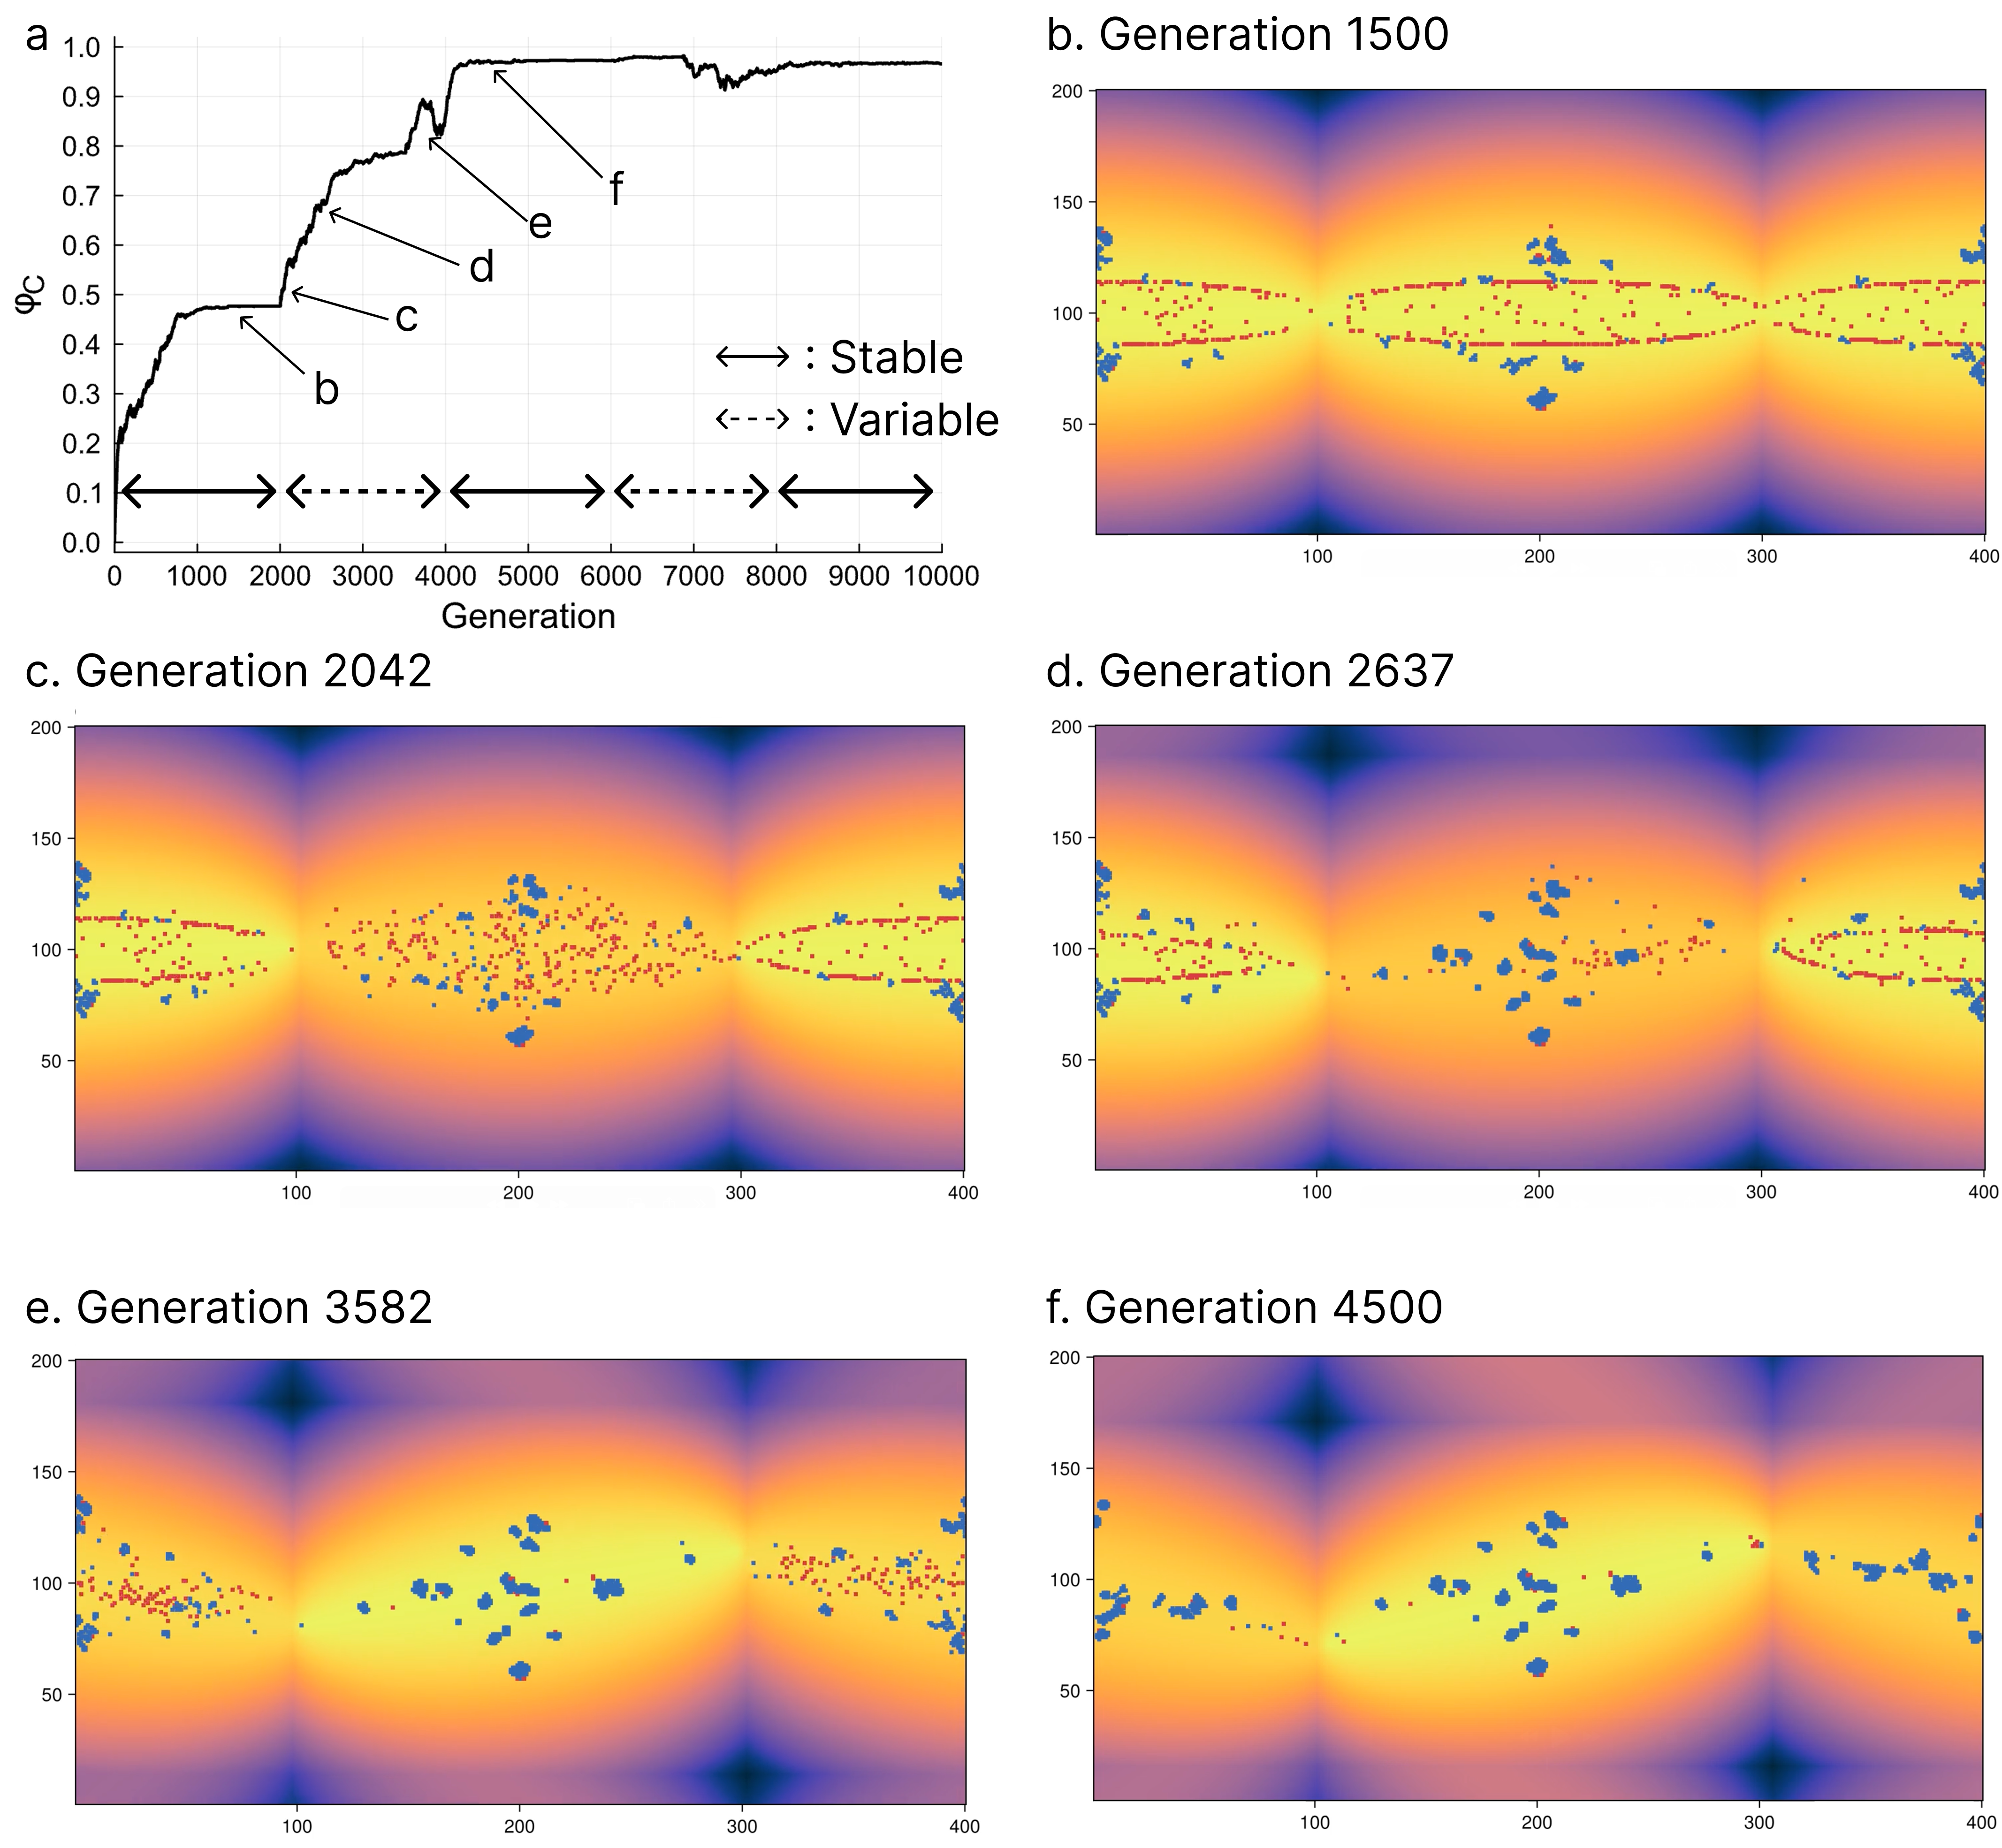
\includegraphics[width=0.95\linewidth]{figures/2/Fig3}
    \caption[The effect of UV.]{
The effect of UV.
(a) The effect of UV across $b \in [1.0, ..., 2.0]$ and $\sigma_\theta \in [0.1, 0.2]$.
The horizontal axis represents the intensity of UV, $\beta$,
and the vertical axis shows the mean cooperation rate over the last $5,000$ generations across $100$ trials.
(The line color scheme of these lines is same as in Fig \ref{Fig:Regional}a.)
(b) Examples of the cooperation rate transition when $b = 1.8$ and $(\beta, \sigma_\theta) \in [(0.1, 0.1), (0.1, 0.2), (0.9, 0.1)]$.
The horizontal axis represents generations, and the vertical axis shows the cooperation rate.
Higher UV tends to result in the cooperation rate fluctuating at higher levels, but convergence is not observed.
    }
    \label{Fig:Universal}
\end{figure}

\subsection*{Effect of CV}

We then examined the combined effects of both RV and UV.
The results (Fig \ref{fig:combination}) show that, consistent with the separate analyses above, RV strongly promotes the evolution of cooperation, while UV has much subtle effect.

\begin{figure}[ht]
    \centering
    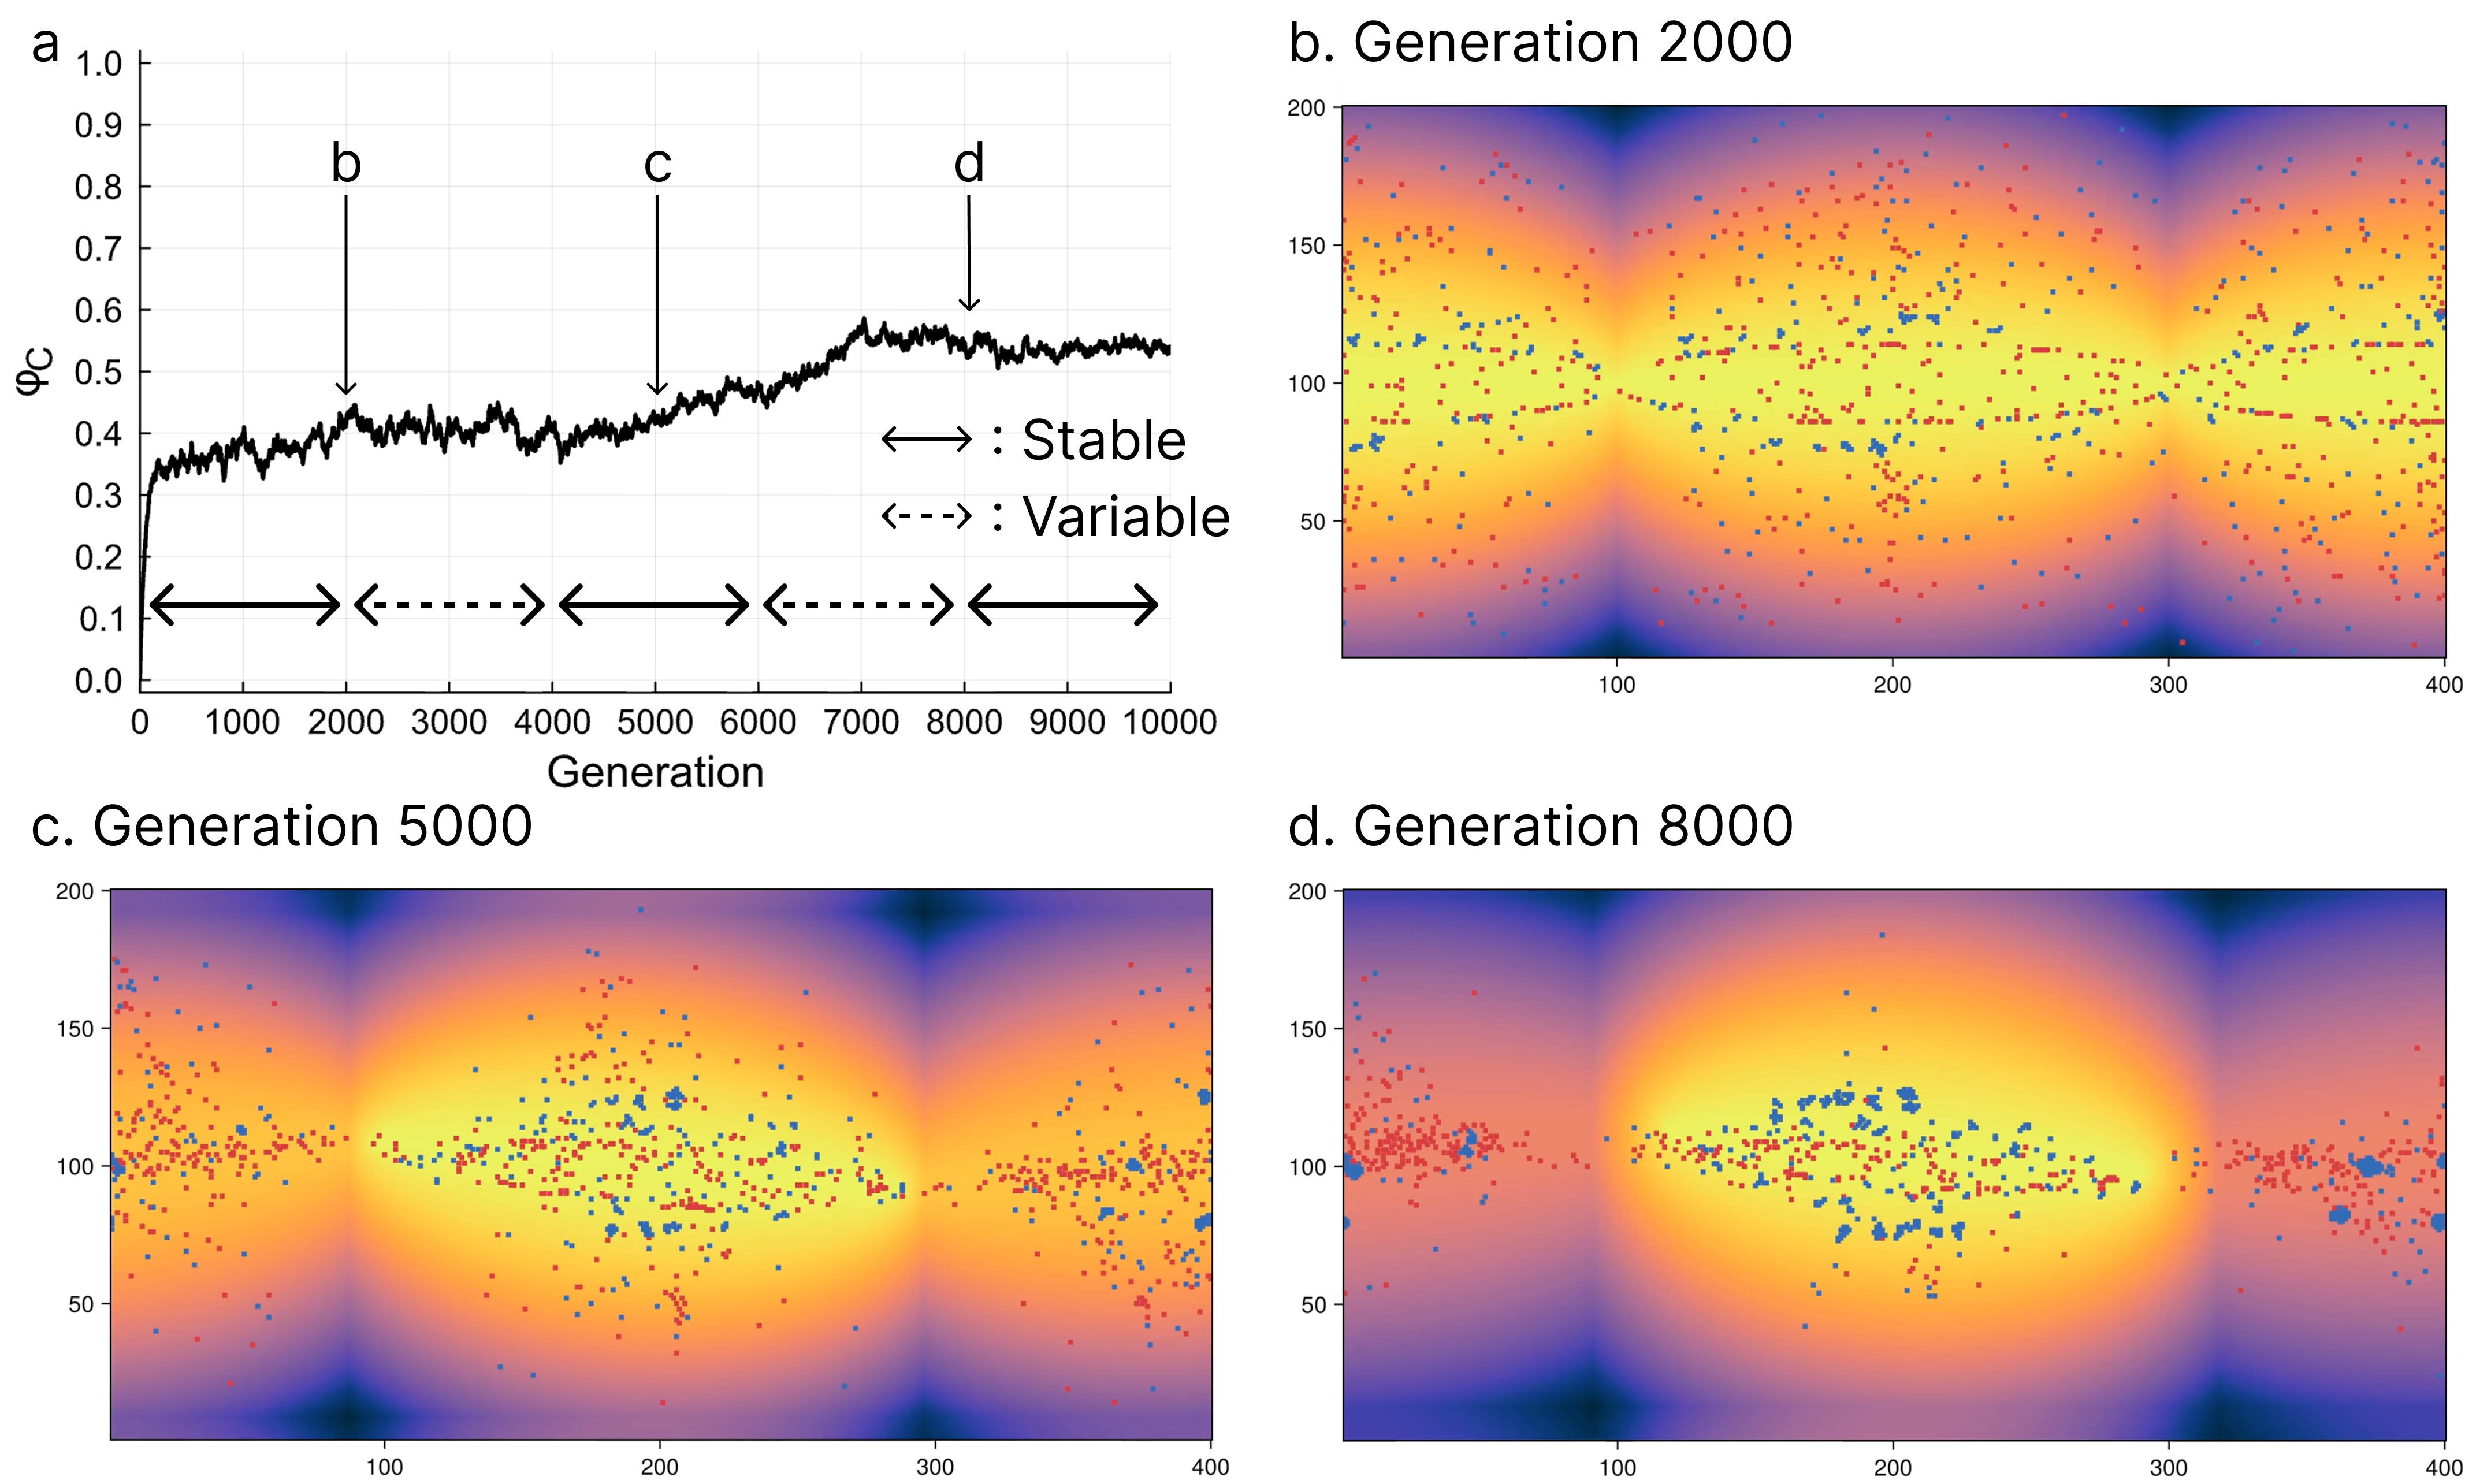
\includegraphics[width=0.95\linewidth]{figures/2/Fig4}
    \caption[The effect of CV ($b = 1.8$).]{
The effect of CV ($b = 1.8$).
(a) and (b) represent cases with $\sigma_\theta = 0.1$, each with a different x-axis.
These plots show that RV increases the cooperation rate significantly, while UV has a limited effect.
(c) and (d) represent cases with $\sigma_\theta = 0.2$, with different x-axis.
The lines are almost flat except in the range $\sigma_R = 0$ to $1$,
indicating that when UV is too high, not only UV but even RV has no effect on the cooperation rate.
    }
    \label{fig:combination}
\end{figure}

\subsection*{Primary drivers of the results}

The results are driven by two key factors:
1. the effects of mutation and EV, which promote fluctuations in cooperation rates, and
2. the coevolution  of cooperation and network structure.

First, RV increases the fluctuations in the cooperation rate, rather than the rate itself.
Fig \ref{fig:mechanism}a shows the effect of EV on strategy distribution in a model that entirely excludes the effects of games and networks.
When these effects are excluded, changes in strategy distribution occur solely due to mutation and strategy updating.
The Y-axis represents the number of agents generated by mutation in one generation, who then serve as role models for strategy updating in the next generation.
These agents are the source of changes in strategy distribution.
The line for RV in the figure shows that as the variability increases, the number of mutated role models increases linearly.
Fig \ref{fig:mechanism}b ``3. (env, C rate)" shows that the time series of RV and the cooperation rate in each of the 100 trials are completely uncorrelated.
Furthermore, the results remain unchanged even when cross-correlation analysis is performed, accounting for time delays.
Therefore, it is evident that RV does not directly affect the cooperation rate but instead promote fluctuations in it.
This can be explained as follows: agents in poorer regions frequently undergo reformations and mutations.
When RV is small, agents rarely accumulate resources in the next generation, causing them to undergo reformations again.
However, when variability is large, agents may become resource-rich in the next generation, and they potentially survive to influence the strategy updates of other agents.
When RV is large, the cooperation rate is more likely to fluctuate up and down.

\begin{figure}[ht]
    \centering
    \includegraphics[width=1.0\linewidth]{figures/2/Fig5.png}
    \caption[Effects of EV on cooperation.]{
Effects of EV on cooperation.
(a) The number of mutated role models as a function of RV and UV.
The simulations are based on a model that excludes games.
Therefore, the figure shows how EV and reformation impact the system without the effect of games or network structure.
(b) Correlation analysis through time series ($10,000$ generations) between variables related to EV
(For RV, env refers to the shift distance of the SoR per generation; for UV, env refers to the value of threshold $\theta$),
network structure (degree SD: standard deviation of degrees, hub count: number of nodes with a degree of $10$ or more), and
cooperation (C rate: frequency of C, resource diff: the difference in average resources between C and D, and degree diff: the difference in average degree between C and D).
The mean correlation coefficients are averaged over $100$ trials for both RV and UV.
$b = 1.8$ for all simulations, $\sigma_R = 16$ for RV, and $\beta = 0.7$, $\sigma_{\theta} = 0.1$ for UV.
}
    \label{fig:mechanism}
\end{figure}

Notably, the analytical solution (\ref{eq:n_MR}) aligns closely with the simulation results for RV shown in Fig \ref{fig:mechanism}a.
\begin{align}
E[n_{MR}] &= \sum_{k=0}^n \mu^k (1 - \mu)^{n - k} k \frac{\sigma_R}{N} \notag \\
          &= \frac{n \mu}{N} \sigma_R \label{eq:n_MR}
\end{align}
In this equation, $E[n_{MR}]$ denotes the expected number of mutated role models, which are generated through mutation and later serve as role models for the strategy updates of other agents.
The right-hand side of the equation represents the expected number of mutated agents within a population of reformed agents, $n$, weighted by the effect of RV, $\sigma_R$, across the entire agent population, $N$.
This equation is simplified by applying the formula for the expectation of a binomial distribution.

Second, once the cooperation rate increases, it is likely sustained through the coevolution of cooperation and network structure.
Fig \ref{fig:mechanism}b 7 indicates that the cooperation rate is correlated with the difference in resources between C and D.
This correlation likely arises because, as the frequency of C increases, mutual support among Cs strengthens, leading to an increase in the average resources of C.
Fig \ref{fig:mechanism}b 8 further shows that the difference in resources is strongly correlated with the difference in network degree between C and D.
This occurs because, in the reformation process of our model, agents with more resources acquire more edges.
Finally, Fig \ref{fig:mechanism}b 6 demonstrates that there is a correlation between the difference in degree and the cooperation rate. This is likely because, as shown in several studies \cite{Santos2005, Santos2006, Santos2008}, heterogeneous degree distributions tend to facilitate cooperation in networks. Thus, a positive feedback loop can form, in which an increase in the cooperation rate induces resource heterogeneity, which subsequently results in network degree heterogeneity, and this network heterogeneity, in turn, reinforces the cooperation rate, which is thought to help sustain the maintenance of a cooperation rate that initially emerged by chance. This explanation is based on correlation and inference, and does not rule out the involvement of other factors.
One possible factor is the influence of resource heterogeneity on strategy update frequency, which has been suggested to promote cooperation \cite{Meng2024}. This process may operate alongside the previously described process where an increase in the cooperation rate widens the resource gap between C and D.

In contrast, UV does not significantly promote cooperation for two reasons:
it fails to generate sufficient fluctuation in the cooperation rate, and
it inhibits the coevolution of cooperation and the network structure.
As shown by the two UV lines in Fig \ref{fig:mechanism}a, increasing variability does not substantially increase the number of mutated role models, unlike the linear relationship seen with RV.
Furthermore, when UV is intense and the threshold $\theta$ becomes very large, almost all agents undergo reformation.
This leads to a reduction in network heterogeneity, which is critical for the coevolution of cooperation and network structure.
This is reflected by the strong inverse correlation between UV and network heterogeneity (Fig \ref{fig:mechanism}b 1-2).
The factors that promote cooperation in RV are ineffective in the context of UV, which explains why UV does not significantly promote cooperation.
When RV and UV are combined in the CV model, the results remain consistent, RV promotes cooperation, while UV has a much smaller effect.

In summary, the observed patterns in cooperation rates can be attributed to the combined effects of mutation and EV, as well as the coevolution of cooperation and network structure.
Specifically, when these two factors work well together, as in the RV model, environmental change promotes cooperation.
However, when the first factor is weak and inhibits the second, as in the UV model, cooperation is less likely to evolve.

\section*{Discussion}

Building on Potts's VSH \cite{Potts1996, Potts1998}, we explored the effects of EV through two simplified models: RV and UV models.
Our results show that RV clearly promotes the evolution of cooperation, while UV has a much smaller effect.
The reason RV fosters cooperation is that it disrupts the distribution of strategies, and the cooperative states that occasionally emerge from these disturbances are sustained by the coevolution of cooperation and network structure.
In contrast, UV does not significantly promote cooperation because the disturbances it causes are insufficient and because it hinders the evolution of the network structure.
Even when both RV and UV are combined, only RV proves effective, with UV having little impact.
Thus, when EV's disturbance effect and the coevolution of cooperation and network structure align, EV facilitates the evolution of cooperation.
However, EV does not promote cooperation if it fails to create sufficient disturbance in strategy distribution or if it undermines the network’s heterogeneous structure.

Our study offers a new perspective on the evolution of cooperation and has the potential to guide future research on modern human behavior in archaeological contexts.
First, although some research on the evolution of cooperation considering EV has been conducted in biology and physics \cite{Brockhurst2007, Miller2015, Gokhale2016, Stojkoski2021, Assaf2013}, few studies have approached it from an anthropological perspective.
To address this gap, we offer a novel explanation for how EV may influence cooperative behavior, using a model that simulates interactions among human groups during the MSA.
Notably, we also identify a key condition for EV to promote cooperation: cooperation and network structure must coevolve effectively.
Second, our findings suggest that the VSH, which has primarily been linked to the CBH, may also be connected to the SBH, thus expanding the scope of VSH.
The conventional CBH explanation \cite{Potts1996, Potts1998, Schuck-Paim2008, Sol2008, Sol2009} is that the brains of the ``versatilists," evolved to rapidly adapt to new environments under EV, contributing to the development of modern human behavior.
In contrast, our novel interpretation, linking EV to SBH, suggests the following sequence.
EV promotes intergroup cooperation, as demonstrated in our study.
The cooperation likely leads to the emergence of more complex, interdependent societies, which introduce new social challenges such as communication, coordination, and conflict resolution across group boundaries.
The increasing complexities of these societies exerts selection pressure on cognitive abilities, favoring individuals who are better equipped to navigate these dynamics.
Over time, this process likely drives the evolution of modern human behavior, characterized by advanced intellectual abilities and complex social structures.
Finally, not previously mentioned, our network model, which incorporates both relationship and geographical structures, can be viewed as a type of multiplex network \cite{Wang2015}.
This perspective opens new avenues for mutual enrichment by enabling comparisons between our findings and the extensive body of research on multiplex and multilayer networks \cite{Gomez-Gardenes2012, Wang2015, Su2022a, Inaba2023}, potentially providing deeper insights into the dynamics of cooperation within complex social and spatial frameworks.

Although this study provides valuable insights into the relationship between EV and cooperation, several limitations should be considered for a more comprehensive understanding.
These limitations include the validity of our model in relation to real-world scenarios during the MSA, the extent to which our results explain actuality, and the need for further mathematical analysis.
We have prioritized simplicity in constructing the model; it is essential to verify which aspects align with reality and which do not.
This includes evaluating the EV patterns, geographical structure, population and grouping dynamics, the specifics of intergroup interactions (game), and the mechanisms through which collective behaviors propagate (reformation), as influenced by empirical research.
An important aspect of intergroup interactions that our current model does not account for is an interaction model biased by the memory of past cooperation and exploitation. This extension, which assumes that agents interact more frequently with those who have previously cooperated with them while avoiding those who have not, could provide insights into the emergence of more complex social structures.
Meanwhile, as our model focuses on the effects of resource variability, neighbor selection is driven by resource availability. However, in reality, the network is also shaped by exogenous and random factors. Models incorporating such factors, known as temporal networks \cite{Holme2012, Li2020, Masuda2020}, have received growing attention. Future extensions accounting for these factors may provide new insights and broaden our research scope.
Additionally, population changes and mobility must be considered, and we plan to address mobility in future work.
We also need to wait for future empirical studies to assess how well our results correspond to the actual events of the MSA.
Furthermore, mathematical analysis is required to better understand the conditions under which EV and other dynamic structures can foster cooperation.
Although the complexity of the phenomenon makes it challenging to propose analytical solutions, theoretical research using simpler models should complement our findings.
Thus, while our study does not aim to establish universal laws, it presents a valuable hypothesis that is expected to guide future theoretical and empirical research in this area.